\section{Formal transformation rules}
In this section we will describe how we may transformation a single line of modules in a configuration into other configurations which may be more efficient. In the first section we describe some basic mathematical sets that are used to describe the transformation rules in the following subsections.

\subsection{Common sets} 
In this section we will try to define a factory configuration using mathematical sets. The sets presented here are used to explain transformation rules in the following subsections.

Previously we presented recipes as acyclic dependency graphs. However at this level of abstraction we do not require the order in which works must be performed. Thus a recipe is simply defined as the set of works needed to be performed on it: 

\[recipe: \textit{A set of all work required to be done by a concrete recipe}\]

A factory configuration is made up of modules. Each module is defined by the following tuple:

\[module: \textit{(aW, mW, up, right, down, left, shadow)}\]

\noindent Where each element of the tuple represents the following:
\begin{itemize}
\item $aW$: The set of work that the module is actively doing.
\item $mW$: The set of work that the module can do.
\item $up,\, right,\, down,\, left$: Describes connections in one of four directions. Each can be either another module or $\emptyset$.
\item shadow: a boolean indicating whether there is a module placed above or below the module.
\end{itemize}

This definition closely resembles our previous definition of a module. Yet, we add $aW$ as to simplify the logic of our rules. 


In \cref{fig:trivial-example} we see that a configuration is made up of a single line of modules, while \cref{fig:running-example} is made up of three. As such we would like to define a factory configuration as a set of lines of modules, where the flow in each line is moving from left to right.

Let us define a line as a set of modules, which are ordered on the $\prec$ relation. This relation takes two modules $m_1$ and $m_2$ as arguments. It evaluates to true if there is a path from $m_1$ to $m_2$ in the actual factory configuration when we only traverse rightwards. $\prec$ is a total order, and we can thus define a line as a totally ordered set of modules, ordered using $\prec$:

\[line: \textit{A total ordered set of modules ordered on } \prec\]

Having defined recipes, modules and lines we choose to define a factory configuration with the following tuple. 

We now define a configuration as the following tuple:

\[configuration: (R, M, \Gamma)\]

Where:
\[R: \textit{The set of all recipes}\]
\[M: \textit{Set of all modules}\]
\[\Gamma: \textit{The set of all lines}\]


Furthermore we only want each $module$ to appear in a single $line$. To enforce this we set up the following rule for each $line$ $\gamma$, in $\Gamma$:
\[\texttt{if } \gamma \in \Gamma \texttt{ then } \forall m \in \gamma \land \forall \gamma ' \in \Gamma \land \gamma \neq \gamma ',\, m \notin \gamma ' \]


We also set up the following rule for each $module$ $m$ in $M$. This is done to ensure that the module can not perform work not within a recipe, and that the work which it actively performs should be a part of its total set of works:
\[\texttt{if } m \in M \texttt{ then } m.aW \subseteq m.mW \land m.mW \subseteq  \bigcup_{r\in R}r\] 

We also need to describe that not all available modules need to be a part of our factory configuration. There may exist free modules, which are not used, but may aid in the search for a higher throughput. First we describe the set of all modules used by a configuration, denoted $CM$:

\[CM = \{m \in \gamma | \gamma \in \Gamma \}\]

The set of free modules $FM$ is then given by:

\[FM = M \setminus CM \]


\subsection{Anti-Serialization}
In this section we will describe a set of transformation rules known as Anti-Serializations. In \cref{fig:trivial-example} all items made according to the three recipes in \cref{fig:toy-recipes} will have to pass through modules, which do not work on them. We would like to minimize this as to reduce the total length that each item must be transported, in addition to combating bottlenecks on the line. Thus it would be beneficial if items could bypass modules that do not work on them. We get around this by branching out production on more lines, where items only go through modules that work on them. 

\subsubsection{$AS_0$: Branch Between Common Modules}
We start by defining the most common type of anti-serialization with the $AS_0$ transformation rule given in \cref{def:as0}. Informally the rule states that if we have a set of modules $B_{r,s,e}$, which works the recipe $r \in R$ exclusivly, lying between the modules $s$ and $e$ on $\Gamma_0$ then we may branch out all modules in $B_{r,s,e}$ to form a new line. This new line is connected to $\Gamma_0$ at $s$ and $e$. We will explain this more in depth, by going over the sets brough up in the rule. 

\begin{definition}[htb]
\runatt{AS}{0}
    \infrule
        {0 < |B_{r,s,e}| \land  s <_k e}
        {(R,M,\Gamma, \Gamma_0, AW, Start, End) \rightarrow_{AS}
        (R,M,\Gamma', \Gamma_0', AW, Start', End') } \\
        Where: \\
        $r \in R$ \\
		$s,e \in K_{\Gamma_0,r}$\\		
		$\Gamma_0' = (Pre_s \cup \{s\}  \cup A_{r,s,e} \cup \{e\} \cup Pos_e, \prec)$ \\     
        $\Gamma' = (\Gamma \setminus \{\Gamma_0\}) \cup \{\Gamma_0'\} \cup B_{r,s,e} $ \\
		$Start' = Start \cup \{(B_{r,s,e}, s)\}$ \\
		$End' = End \cup \{(B_{r,s,e}, e)\}$

\caption{Formal definition of the $AS_0$ transformation rule}
\label{def:as0}
\end{definition}

We initially define a special set on $r$, $\bar{r}$, which contains all types of work which are not unique to $r$:
\[\bar{r} = \bigcup_{r' \in R}r', \texttt{ if } r' \neq r\]

Next we define, what we refer to as common modules. These are modules in $\Gamma_0$, which $r$ needs to use along with at least some other recipe. These are important to identify, as they may not be branched out, as that would make them inaccessible to the other recipes than $r$.  Given $r$ and $\Gamma_0$ we define the set of common modules $K_{\Gamma_0,r}$ as follows:

\[K_{\Gamma_0 ,r} = \{m | m \in \Gamma_0  \land \exists \rho \in AW(m),\, \{\rho\} \subseteq r \land \{\rho\} \subseteq \bar{r} \land r \in R\}\]

From this set we can then define $\alpha_{\Gamma_0 ,r}$, which is the set of modules in $\Gamma_0$ which are not used by $r$: 

\[\alpha_{\Gamma_0 ,r}  = \{m |m \in \Gamma_0 \land \forall \rho \in AW(m),\, \{\rho\} \nsubseteq r \land r \in R\}\]

Along with $\beta_{\Gamma_0 ,r}$, which is the set of modules in $\Gamma_0$ used only by $r$:

\[\beta_{\Gamma_0 ,r}  = \{m  | m \in \Gamma_0 \land \forall \rho \in AW(m),\, \{\rho\} \subseteq r \land \{\rho\} \nsubseteq \bar{r} \land r \in R\}\]

Next we define the binary relation relation $<_K$ as:
\[a <_K b = \left\{\begin{matrix}
tt \texttt{ if } a,b,c \in K_{\Gamma_0 ,r} \land a \prec b \land \lnot (a \prec c \land c \prec b) \\ \texttt{else } ff
\end{matrix}\right.\]

We also define a total order of all modules in between two modules, $s$ and $e$, in some line $\gamma \in \Gamma$:

\[M_{s,e} = (\{m | m \in \gamma \land \gamma \in \Gamma \land s \prec m \land m \prec e\}, \prec)\]

We can now define the total order of all modules appearing between $s$ and $e$, which are not used to work $r$, $A_{r,s,e}$ as follows: 

\[A_{r,s,e} = (\{m |m \in M_{s,e} \land m \in \alpha\}, \prec)\]

Similarly we can define the total order $B_{r,s,e}$, which contains all modules that appear between $s$ and $e$ which work exclusivly on $r$

\[B_{r,s,e} = (\{m |m \in M_{s,e} \land m \in \beta\}, \prec)\]

We define $Pre_{s}$ which is the set of all modules that come before a module $s$ in line $\gamma \in \Gamma$:
\[Pre_{s} = (\{m | m \in \gamma \land \gamma \in \Gamma \land m \prec s\}, \prec)\]

And lastly we define $Pos_{e}$ which is the set of all modules that come after a module $e$  in line $\gamma \in \Gamma$:
\[Pos_{e} = (\{m | m \in \gamma \land \gamma \in \Gamma \land e \prec  m \}, \prec)\]

Having defined these sets the rule in \cref{def:as0}, shows that in the case where $|B_{r,s,e}| > 0 \land s <_K e$ then we may update $\Gamma$ with two new lines, including an update of $\Gamma_0$ that describes a branch out from $\Gamma_0'$, which exclusivly works upon $r$ before rejoining with the old line.   

While this rule is formally sound it can be difficult to read. As such we have tried to illustrate the transformation from configuration to configuration visually in \cref{fig:as0}. This visualization uses a homemade notation. Square boxes refer to individual modules. Boxes with rounded corners are total orders of sets of modules. A graphical line of boxes flowing from left to right is a line in $\Gamma$ ordered as shown. If a module $s$ and a line $\gamma$ are connected by a vertical upward going edge, then $Start$ contains the ordered pair $(\gamma ,s)$. At the same time, if the edge goes downwards from a line $\gamma$ to a module $e$, then $End$ contains the ordered pair $(\gamma ,e)$.

%A box with rounded corners containing "..." means that here is a total order of one or more modules, but we do not care what they contain.

\begin{figure}[H]
\centering
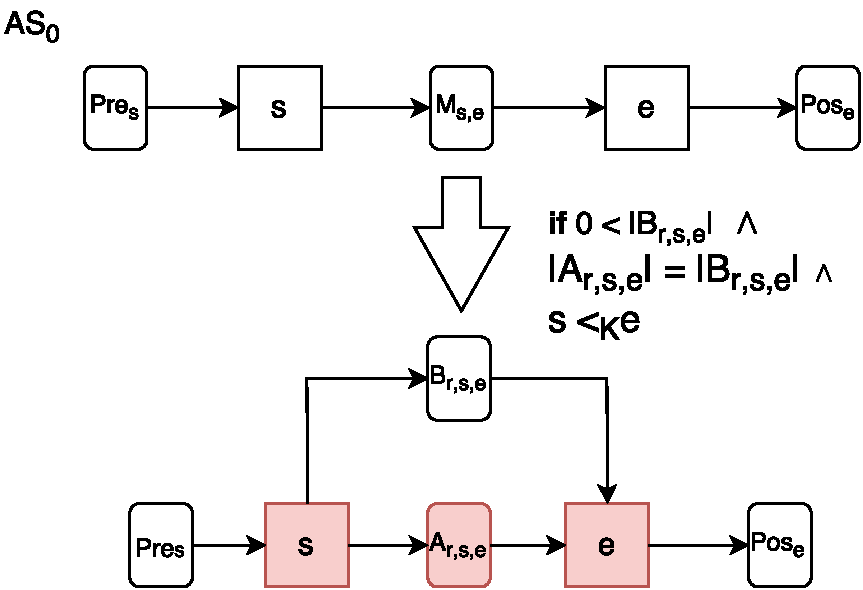
\includegraphics[width=\textwidth]{as0.pdf}
\caption{A visual representation of the $AS_0$ transformation rule}
\label{fig:as0}
\end{figure}

For the rest of this section, we will now use these visualization for explaining our transformation rules, instead of setting up transition rules. If any new derived sets are shown in a new transformation rule, we will describe them as well.  

In the rest of this sub-section we will describe two special cases known as $AS_1$, branch in, and $AS_2$,  branch out. 

\subsubsection{$AS_1$: Branch In}\label{sssec:bi}
It may be that we have modules that precede the first module of $K_{\Gamma_0 ,r}$ that we would like to branch out, but can't with the rule described in \cref{def:as0}, as it requires two distinct $K_{\Gamma_0 ,r}$ modules. So for this we describe the transformation rule $AS_1$, which can be seen in \cref{fig:as1}.

\begin{figure}[H]
	\centering
	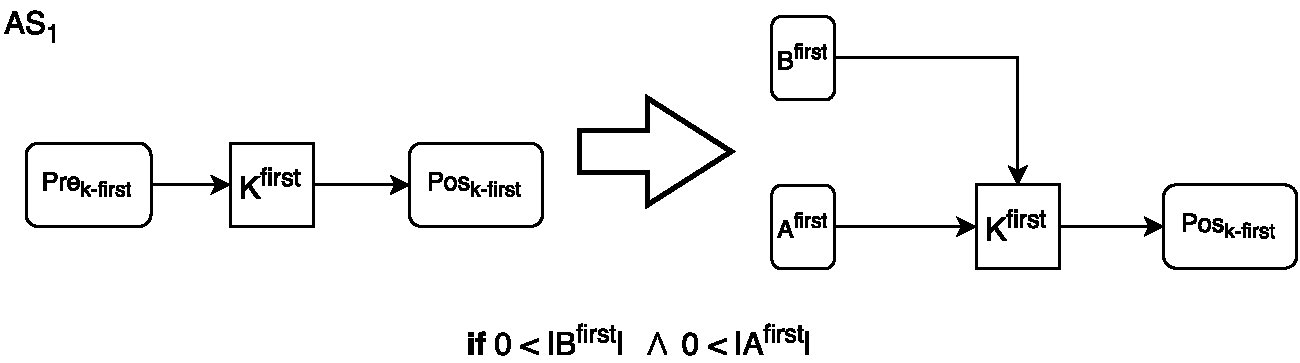
\includegraphics[width=\textwidth]{as1.pdf}
	\caption{A visual representation of the $AS_1$ transformation rule. This is used for the case where we which to branch out modules prior to the first element of $K_{\Gamma_0 ,r}$}
	\label{fig:as1}
\end{figure}


 We define the first module in $K_{\Gamma_0 ,r}$ as:

\[K_{\Gamma_0 ,r}^{first} = m \texttt{ where } \forall m' \in K_{\Gamma_0 ,r} \land m \neq m',\, m \prec m' \] 

Similarly for the $AS_0$ transformation rule, we define two total orderings. $A_{\Gamma_0 ,r}^{first}$ that describes all modules before $K_{\Gamma_0 ,r}^{first}$ on which $r$ does not perform any work. And $B_{\Gamma_0 ,r}^{first}$ which describes all modules before $K_{\Gamma_0 ,r}^{first}$ on which $r$ exclusively works.

\[ A_{\Gamma_0 ,r}^{first} = (\{m | m \in \alpha_{\gamma ,r}  \land m \in Pre_{K_{\Gamma_0 ,r}^{first}} \}, \prec) \]

\[ B_{\Gamma_0 ,r}^{first} = (\{m | m \in \beta_{\gamma ,r}  \land m \in Pre_{K_{\Gamma_0 ,r}^{first}} \}, \prec) \]

We also again use the $Pre_s$ and $Pos_e$ sets here, but used on $K_{\Gamma_0 ,r}^{first}$ instead of $s$ and $e$.
  

\subsubsection{$AS_2$: Branch Out}
Similarly to $AS_1$ we have the case where the last element in $K_{\gamma ,r}$, is proceeded by a set of modules that we would like to branch out. For this we describe the transformation rule $AS_2$, which can be seen in \cref{fig:as2}.

\begin{figure}[H]
	\centering
	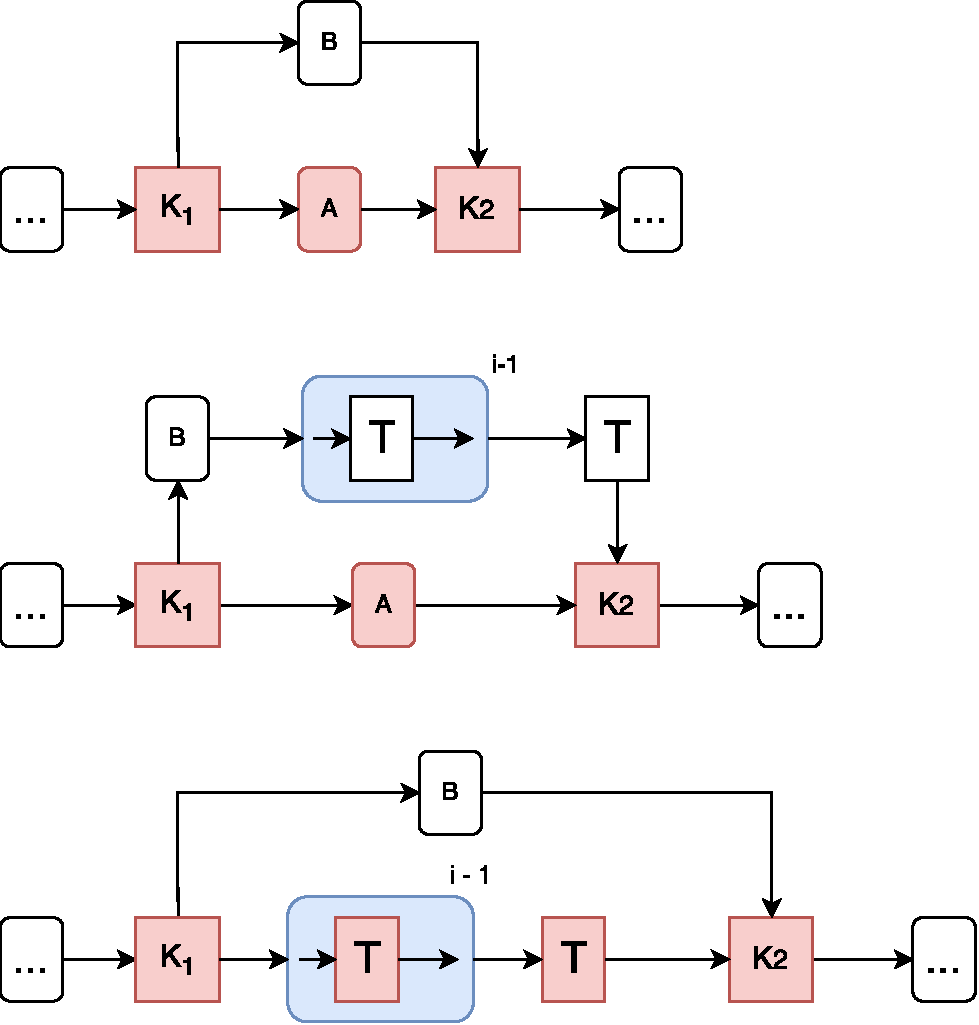
\includegraphics[width=\textwidth]{as2.pdf}
	\caption{A visual representation of the $AS_2$ transformation rule. This is used for the case where we which to branch out modules proceeding the last element of $K_{\Gamma_0 ,r}$}
	\label{fig:as2}
\end{figure}


We define the last module in $K_{\Gamma_0 ,r}$ as:

\[K_{\Gamma_0 ,r}^{last} = m \texttt{ where } \forall m' \in K_{\Gamma_0 ,r} \land m \neq m',\, m' \prec m \] 


Again we also define two total orders. $A_{\Gamma_0 ,r}^{last}$ that describes all modules after $K_{\Gamma_0 ,r}^{last}$ on which $r$ does not perform any work. And $B_{\Gamma_0 ,r}^{last}$ which describes all modules after $K_{\Gamma_0 ,r}^{last}$ on which $r$ exclusively works.


\[ A_{\Gamma_0 ,r}^{last} = \{m | m \in \alpha_{\gamma ,r}  \land m \in Pos_{K_{\Gamma_0 ,r}^{last}} \} \]

\[B_{\Gamma_0 ,r}^{last} = \{m | m \in \beta_{\gamma ,r}  \land m \in Pos_{K_{\Gamma_0 ,r}^{last}} \}\]



%\subsubsection{Restricting branches}
%For the previous transformation rules, we have imagined that no other branch has been made from our line to any side. Yet, this will not always be the case. To be flexible enough to produce configurations with high throughput, we need to handle this. We go more in depth with how to enforce some general physical rules in \cref{ssec:conflicts}, but here we will tackle one unique to anti-serialization.

%On the top part of \cref{fig:shadowexample}, we see that we have already made a branch from $s1$ to $e1$, which results in the modules on the old being shadowed. Being shadowed means that if we remove the module and just reconnect the old line as usual, then the branch becomes too long to connect back to its old line. The line needs to connect back to its designated point on the old line as the module located here is a common module. It performs work on the recipe $r$ otherwise worked on by the new line and should therefore not be bypassed.  To get around this we, as shown in \cref{fig:shadowexample}, alter our anti-serialization transformation in this case to replace a shadowed module with a transport module, as not to skew the two previous lines away from each other. The example shows this done for a single module, but it may be done regardless of the amount of shadowed modules which we remove.

%We may however not do this if the shadowed module is also a module where a branch either connects from or to. This means that the module is common and is used by the branch. Removing it would keep us from producing that branch's specific recipe. Therefore we never allow for these modules to be removed, even if this means that we can not perform certain anti-serializations.

%\begin{figure}[H]
%\centering
%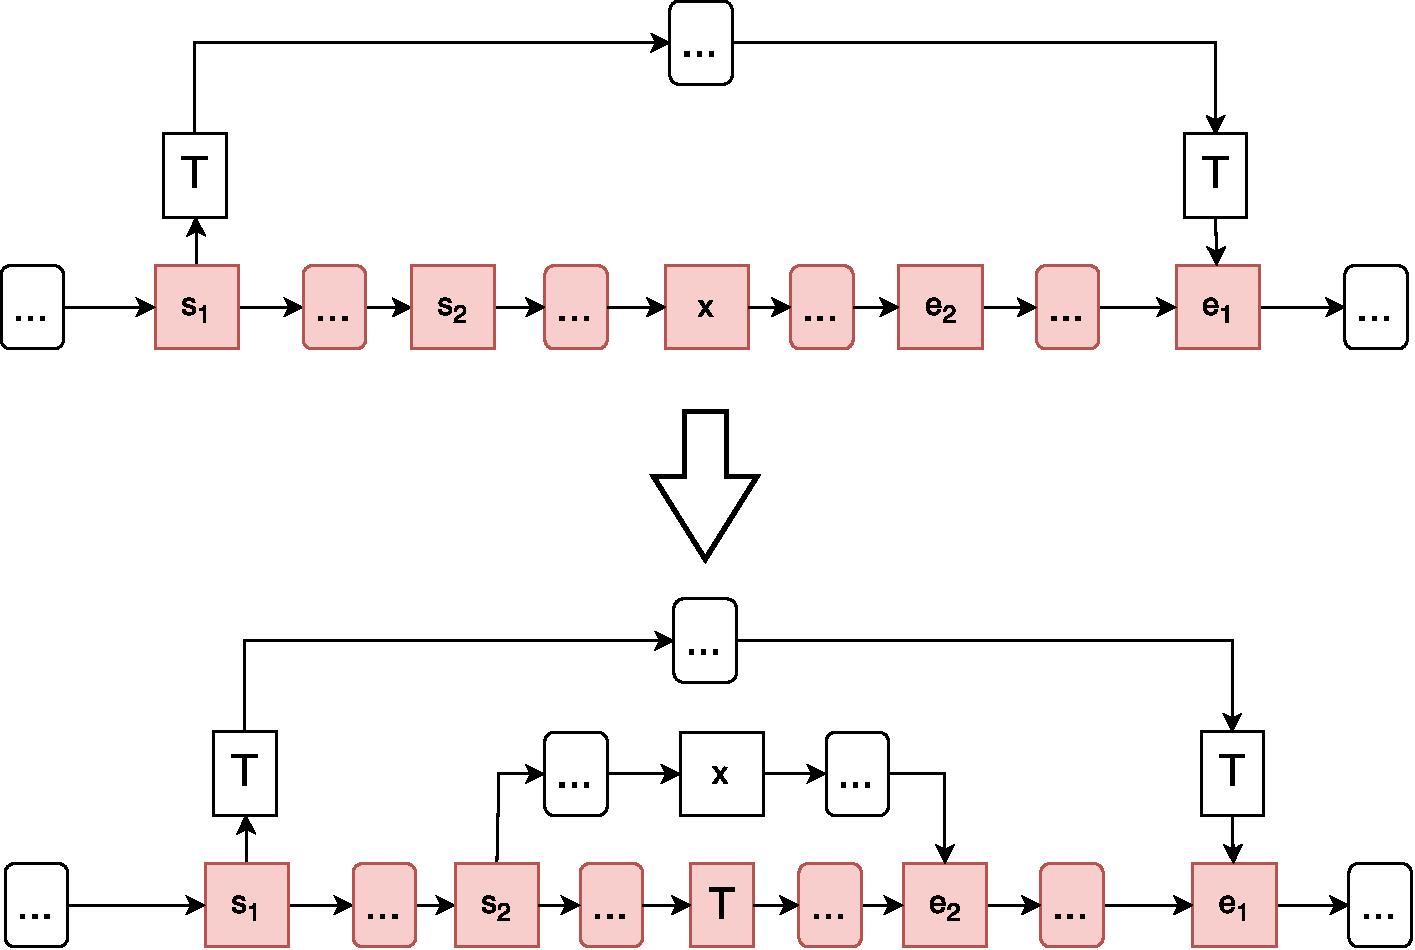
\includegraphics[width=\textwidth]{as5.pdf}
%\caption{Transformation that handles the case where an %anti-serialization removes a shadowed module}
%\label{fig:shadowexample}
%\end{figure}


%Now imagine the situation in \cref{fig:asbase}. Here we have specific $s$ and $e$ modules chosen on a line $\gamma$ and we have chosen to branch out a specific recipe $r$. Between the two modules we may have $M_{s,e}$ placed. From this we can calculate $A_{s,e}$ and $B_{s,e}$ as described before. If $B_{s,e} = \emptyset$ then we may branch out some modules only used to work on $r$. 

%If $|A_{s,e}| = |B_{s,e}| + 2$ , then we can branch out as shown in the top of \cref{fig:astrans}. Here we simply remove $|B_{s,e}|$ from the rest of $M_{s,e}$ leaving us with in its place $A_{s,e}$. The module $s$ is then connected upwards to the first element of $|B_{s,e}|$. The last element of $|B_{s,e}|$ is then connected to $e$. This transformation also entails that all of  $|B_{s,e}|$ is removed from $\gamma$ and that a new line containing $|B_{s,e}|$ is added to $\Gamma$. For each of the transformations presented in this subsection we alter $\gamma$ and add to $\Gamma$ the new branch which is created.  Notice that the modules beneath the new line are marked as red. This means that the shadow variable in the module tuples on the old line have been set to true. This is used in order to handle transformation conflicts as described later in \cref{ssec:tc}.

%In the middle of \cref{fig:astrans} we describe the case where $A_{s,e}| > |B_{s,e}| + 2$. The difference between the cardinality of these two sets is called i.  In this case we can not physically connect the last element of $|B_{s,e}|$ downwards to $e$. We get around this issue by appending the new line with i new transport modules. These are modules which can not perform any work and are only used to transport recipes. The last of these transporters is then connected downwards to $e$. The new line added to $\Gamma$ consists of the modules in $|B_{s,e}|$ ordered behind the new transport modules as depicted in the figure. 

%The last case, shown in the bottom of \cref{fig:astrans} is similar to the previous one, but instead $A_{s,e}| < |B_{s,e}| + 2$. In this case we append the original line with transporters instead. This requires an update of $\gamma$ to include these new transporters, while the new line added to $\Gamma$ is again just $|B_{s,e}|$. 

%\begin{figure}[H]
%\centering
%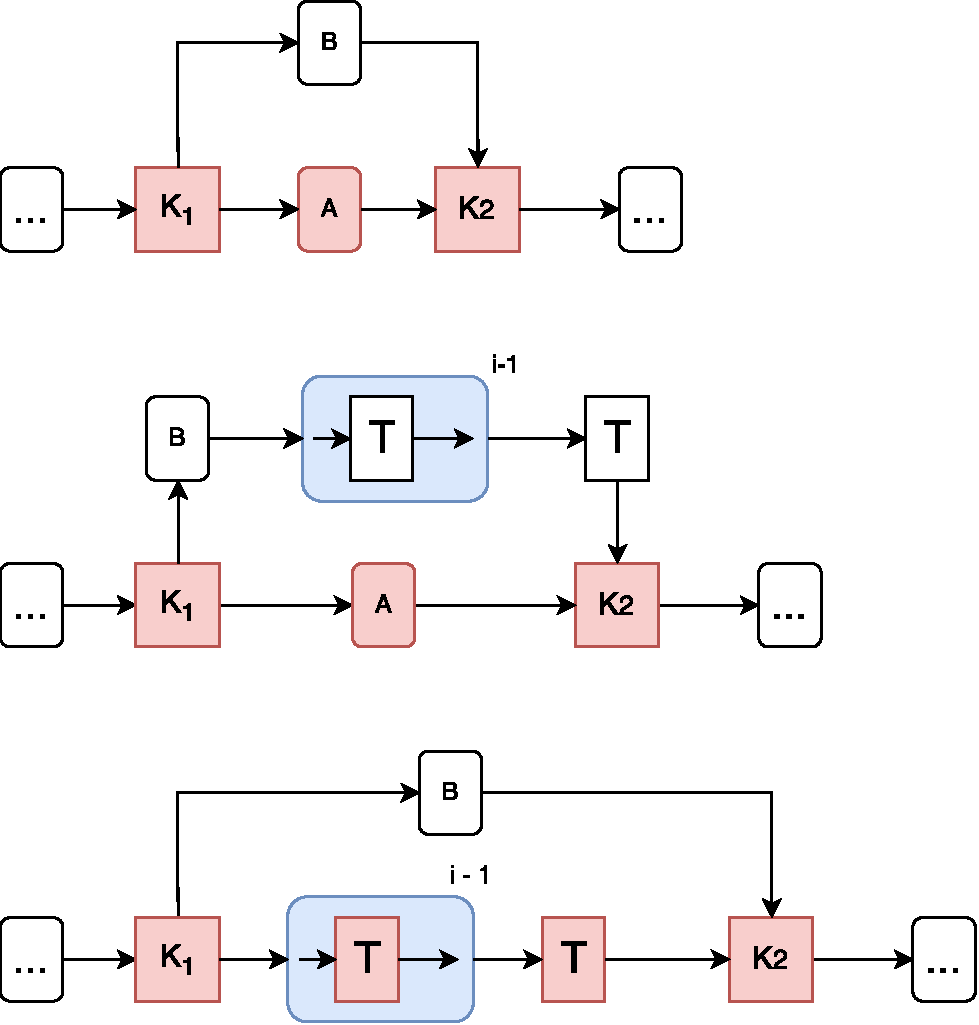
\includegraphics[width=\textwidth]{as2.pdf}
%\caption{3 different configurations to which we may go from %\cref{fig:asbase}. Top: Case when $A_{s,e}| = |B_{s,e}| + 2$. Middle: Case when $A_{s,e}| > |B_{s,e}| + 2$. Bottom: Case when $A_{s,e}| < |B_{s,e}| + 2$ }
%\label{fig:astrans}
%\end{figure}
 
\subsection{Parallel production}
If there are any free modules available that perform work required by your recipes, then it can often be advantages to parallelize certain parts of your configuration using these modules. In this section we will produce a rule for inserting in free modules in order to parallelize certain works. We begin by describing the some required sets.

First we describe the set of pairs, where the first element is a module in between the modules $s$ and $e$ and the second element is a free module that can do atleast the work that the first element is currently doing.
\[Map_{s, e} = \{(m, m')| m \in FM \land m' \in M_{s,e} \land m'.aW \subseteq m.mW\} \]


We then describe all sets of pairs that could be a possible parallel line for the modules between $s$ and $e$. Note that this set could be the empty set, as the modules needed for creating a possible line might not availabe in $FM$.
\[MapPaths_{s,e} = \{p \in {Map}_{s,e}^2 | (m,m') \in p \land (n,n') \in p \land |p| = |M_{s,e}| \land  \forall m': m' \neq n' \}\]

We define $s[1]$ as the operation that given a set of pairs $s$, gives the set of all the first elements of the pairs in $s$.
\[s[1] = \{m_1 | (m_1, m_2) \in s\}\]

Using this we define the set $P_{s,e}$ as $MapPaths_{s,e}$ but without the second element in each pair.

\[ P_{s,e} = \{p[1] | p \in MapPaths_{s,e}\}\]

We can then total order this $P_{s,e}$ using the relation $<_p$ which is defined as follows.

\[a <_{p} b = 
\left\{\begin{matrix}
tt \texttt{ if } x \prec y \land (x, a), (y, b) \in MapPaths_{s,e}\\
\texttt{else } ff
\end{matrix}\right.\]

Now that we have defined these sets we can now describe the rules for parallezing a line in a configuration. We begin with the base case, in which we parallelize everything inbetween two modules. A graphical representation of this can be seen in \cref{fig:para_se}. As shown by the figure, if we can find a $P_{s,e}$ we parallize it by connecting it with transport modules to $s$ and $e$. The order in which $P_{s,e}$ is placed is the total order $(P_{s,e},<_p)$. 

\begin{figure}[h]
\centering
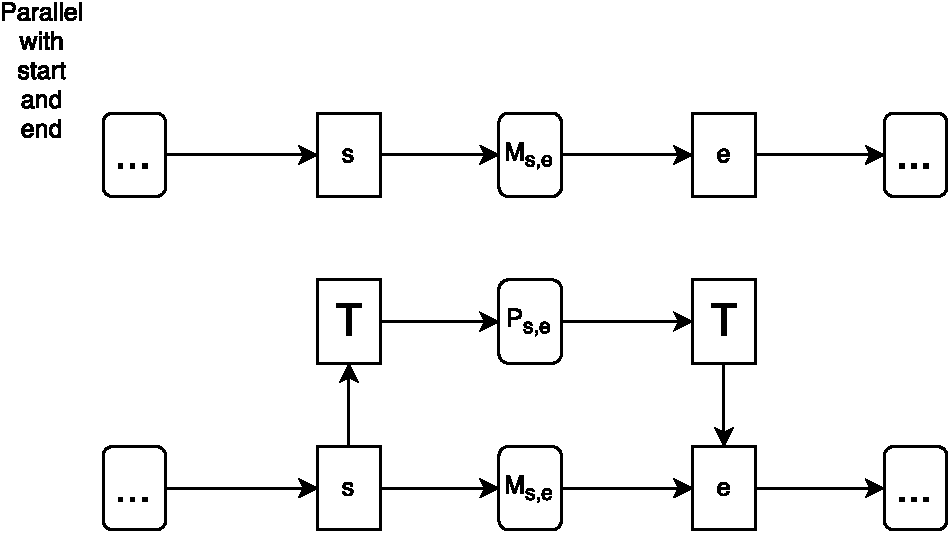
\includegraphics[width=0.5\textwidth]{para_se.pdf}
\caption{Parallelization rule when you have both a start and end module}
\label{fig:para_se}
\end{figure}


We also have two other cases, one in which we have no end module, meaning that we will fork out a parallel line, and the case where we have no start, meaning we will join in a parallel line. A graph showing both of these cases can be seen respectively in \cref{fig:para_we} and \cref{fig:para_ws}. For the case without start we connect the last module in the total order $(P_{s,e}, <_p)$ to $e$, and for the case without end we connect $s$ to the first module the in the total order $(P_{s,e}, <_p)$.


\begin{figure}[h]
\centering
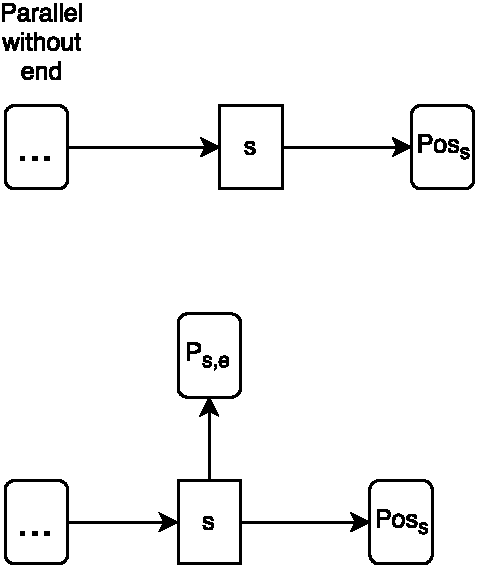
\includegraphics[width=0.3\textwidth]{para_we.pdf}
\caption{Parallelization rule when you do not have an end module}
\label{fig:para_we}
\end{figure}

\begin{figure}[h]
\centering
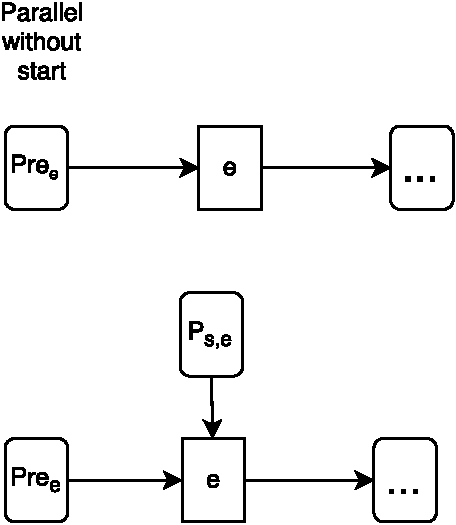
\includegraphics[width=0.3\textwidth]{para_ws.pdf}
\caption{Parallelization rule when you do not have a start module}
\label{fig:para_ws}
\end{figure}

 
\section{Swap}
In this section we will describe a set of transformation rules know as swaps. There are two distinct cases of swaps. One in which we swap out a module in a line with a free module, which is able to do the same work as the one it is replacing is currently doing on some recipe. Second, one in which we swap out a module within a line, and another module within a line that are capable of the same work, which the other is currently doing. These transformations can be beneficial, if we swap a faster module with a slower module at a choke point, allowing for more throughput.

\subsection{$Swap_0$: External Swap}
For the case of swapping a module out from a configuration with a free module, we have described the transformation rule $Swap_0$, which can be seen in \cref{fig:swap0}.

\begin{figure}[H]
	\centering
	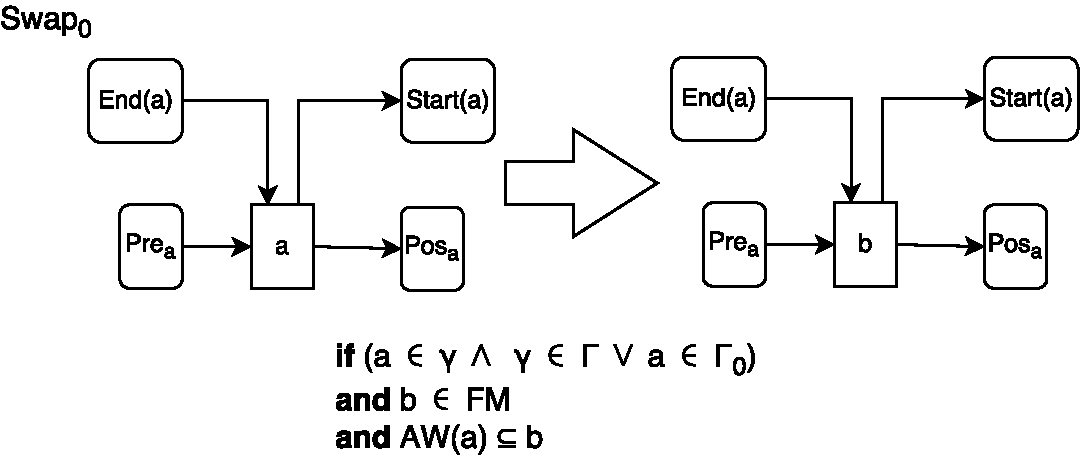
\includegraphics[width=0.7\textwidth]{swap0.pdf}
	\caption{A visual representation of the $Swap_0$ transformation rule}
	\label{fig:swap0}
\end{figure}

Not shown in \cref{fig:swap0} is that we also update the function $AW$ of our new configuration to $AW'$. We define $AW'$ as:

\[AW' = (AW \cup \{(b, AW(a))\} \setminus \{(a, AW(a))\}\]



%We expand our visual representation of our rules with an \texttt{update} clause. This \texttt{update} clause contains a number of update statements, either $add$ and $remove$. The $add$ operation adds a given ordered pair to the function, and the $remove$ operation removes a given ordered pair from the function. An example could be for the function $Foo: X \rightarrow X$ we wish to either add or remove the element $(a, b)$ where $a, b \in X$ then:

%\[Foo.add((a, b)) = Foo \cup \{(a,b)\}\]
%\[Foo.remove((a, b)) = Foo \setminus \{(a,b)\}\]


\subsection{$Swap_1$: Internal Swap}
For the case of swapping a module from a configuration with another module in the same configuration, we have described the transformation rule $Swap_1$, which can be seen in \cref{fig:swap1}.

\begin{figure}[H]
	\centering
	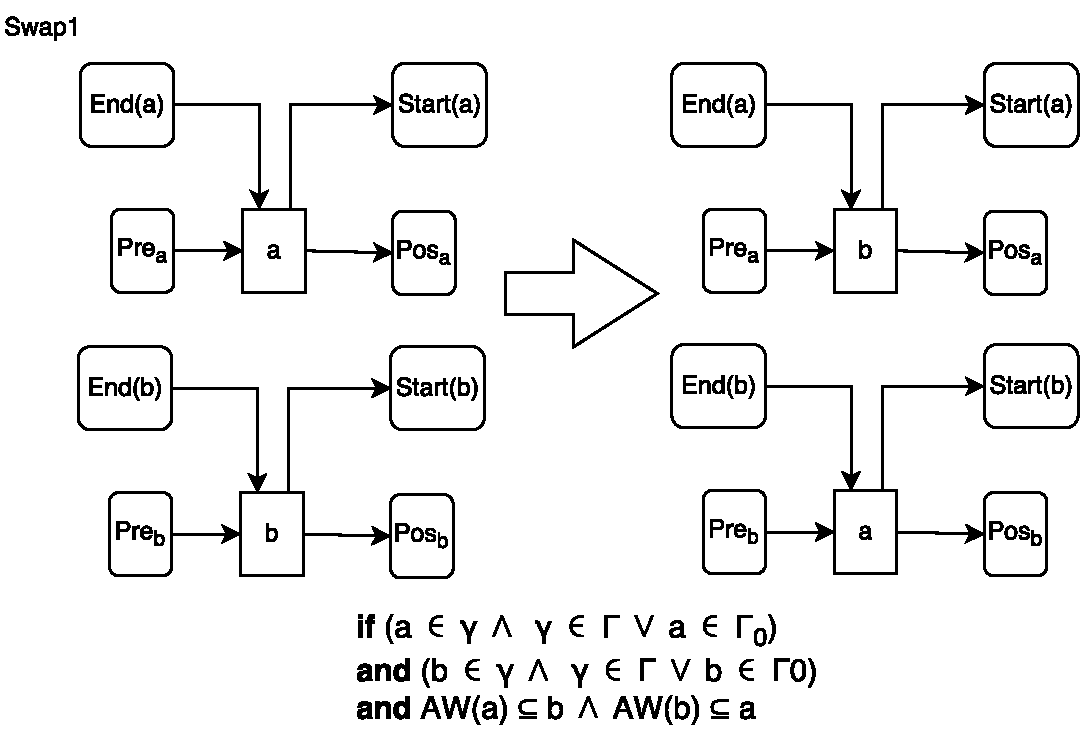
\includegraphics[width=0.7\textwidth]{swap1.pdf}
	\caption{A visual representation of the $Swap_1$ transformation rule}
	\label{fig:swap1}
\end{figure}

Not shown in \cref{fig:swap1} is that we also update the function $AW$ of our new configuration to $AW'$. We define $AW'$ as:

\[AW' = (AW \cup \{(b, AW(a)), (a, AW(b)\} \setminus \{(a, AW(a)), (b, AW(b))\}\]


 
\section{Conflicts}\label{ssec:conflicts}
As mentioned back in \cref{ch:uppaalmodel}, we did not enforce the physical rules of modules to their fullest in the UPPAAL model. These entail that a module may not connect to another module, if this module is not a neighbour and if the connection would force two modules to take up the same space. The anti-serialization transformations rules can currently create configurations, where lacking module connections mean that not all recipes can be fulfilled. This problem will be solved in \cref{ssec:restrictbranch}. Furthermore both our anti-serialization and parallelization rules can cause intersections to occur as a result of adding new lines. We will solve this problem in \cref{ssec:paround} and \cref{ssec:pbeneath}.


\subsection{Restricting Branches Anti-Serialization}\label{ssec:restrictbranch}
For the anti-serialization transformation rules described in \cref{sec:as}, we did not ensure that the first and last elements of the new line can be vertically connected to the $s$ and $e$ modules on the main line. Furthermore, until now, we have imagined that no other branch has been made from our line before performing a transformation. Yet, this will not always be the case, and as such can cause some conflicts.

\subsubsection{Neighbour Errors}
Imagine a situation similar to what the rule $AS_0$ in \cref{fig:as0} describes. Here we have specific $s$ and $e$ modules chosen on the line $\Gamma_0$, and we have chosen to branch out a specific recipe $r$. Between the two modules we have $M_{s,e}$. From this we can calculate $A_{r,s,e}$ and $B_{r,s,e}$ as described before. If $0 < |B_{r,s,e}|$, then we may branch out some modules only used to work on $r$. However in  most cases $B_{r,s,e}$ will not have a size such that it can be connected directly to the $s$ and $e$ modules. We therefore modify our $AS_0$ transformation rule, as to solve this.

If $|A_{r,s,e}| + 2 > |B_{r,s,e}|$ , then the result of our $AS_0$ transformation rule will be the top of \cref{fig:astrans}. In this case, we append the new line with transport modules to make the two lines fit each other. Notice that the modules beneath the new line are marked as shadowed, i.e. coloured red. This is used in order to handle transformation conflicts as described below in \cref{sssec:shadow}. We also introduce blue rounded boxes with indexes to the top right of them. These boxes mean that anything inside of them are serialized $i$ times, where $i$ is the index given with the box. 


If $|A_{r,s,e}| + 2 \leq |B_{r,s,e}|$,  then the result of our $AS_0$ transformation rule will be the bottom of \cref{fig:astrans}, In this case we append \Gamma_0 with transporters instead of the new line as to make them fit together.

\begin{figure}[H]
	\centering
	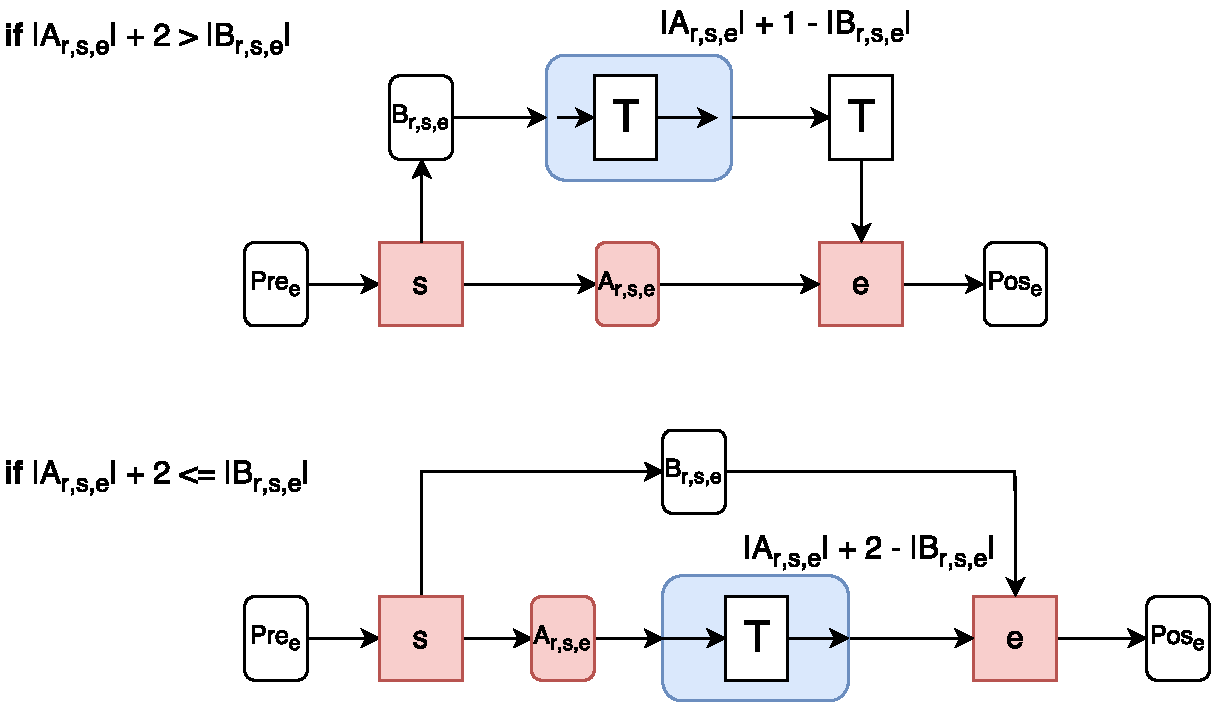
\includegraphics[width=\textwidth]{astrans.pdf}
	\caption{The new results of $AS_0$}
	\label{fig:astrans}
\end{figure}

\subsubsection{Shadowed Modules}\label{sssec:shadow}
On the top part of \cref{fig:shadowexample},  we have already made a branch from $s1$ to $e1$, which results in the modules on \Gamma_0 being shadowed. Being shadowed means that if we remove the module and just reconnect the old line as usual, then the branch becomes too long to connect back to its old line. Shadowed boxes are visualized with the colour red. The line needs to connect back to its designated point on the old line as the module located here is a common module. This module  performs work on the recipe $r$ otherwise worked on by the new line and should therefore not be bypassed. To get around this we, as shown in \cref{fig:shadowexample}, alter our anti-serialization transformation in this case to replace a shadowed module with a transport module, as not to skew the two previous lines away from each other. The example shows this done for a single module, but it may be done regardless of the amount of shadowed modules, which we remove. In \cref{fig:shadowexample} we also introduce rounded boxes with three dots in them. These boxes just means that here appears any number of modules in a total order.

As an exception, we may not remove a shadowed module, if it also used as a branching in or branching out point for some line. This means that the module is common and is used by the branch. Removing it would keep us from producing items according that branch's specific recipe. Therefore, we never allow for these modules to be removed, even if this means that we can not perform certain anti-serializations.

\begin{figure}[H]
	\centering
	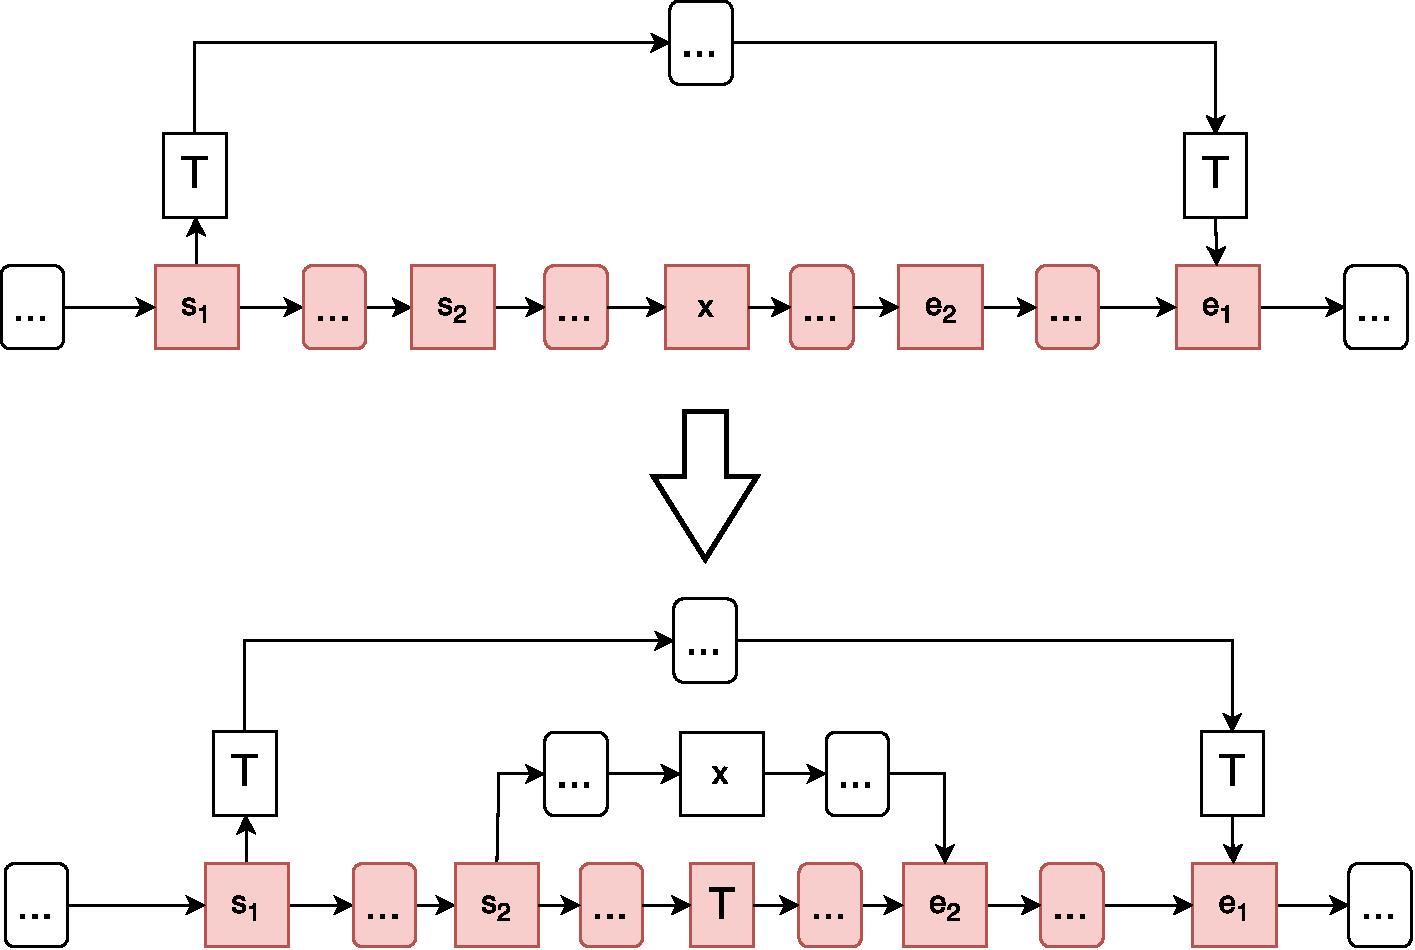
\includegraphics[width=\textwidth]{as5.pdf}
	\caption{Transformation that handles the case where an anti-serialization removes a shadowed module}
	\label{fig:shadowexample}
\end{figure}

\subsection{Push Around} \label{ssec:paround}
In push around we handle the case, where a new off branching line intersects with an old line, by moving the new line above the old line. In the case where the new line entirely covers the old, we perform the transformation depicted in \cref{fig:pusharound1}. As shown, the new line simply uses transport modules to lift itself up above the old line. These transport modules are technically not a part of the line and only serve the purpose of avoiding the intersection. If two modules are connected vertically according to either the $Start$ or $End$ functions, we may add transport modules to ensure that the described vertical path can exist.

\begin{figure}[h]
\centering
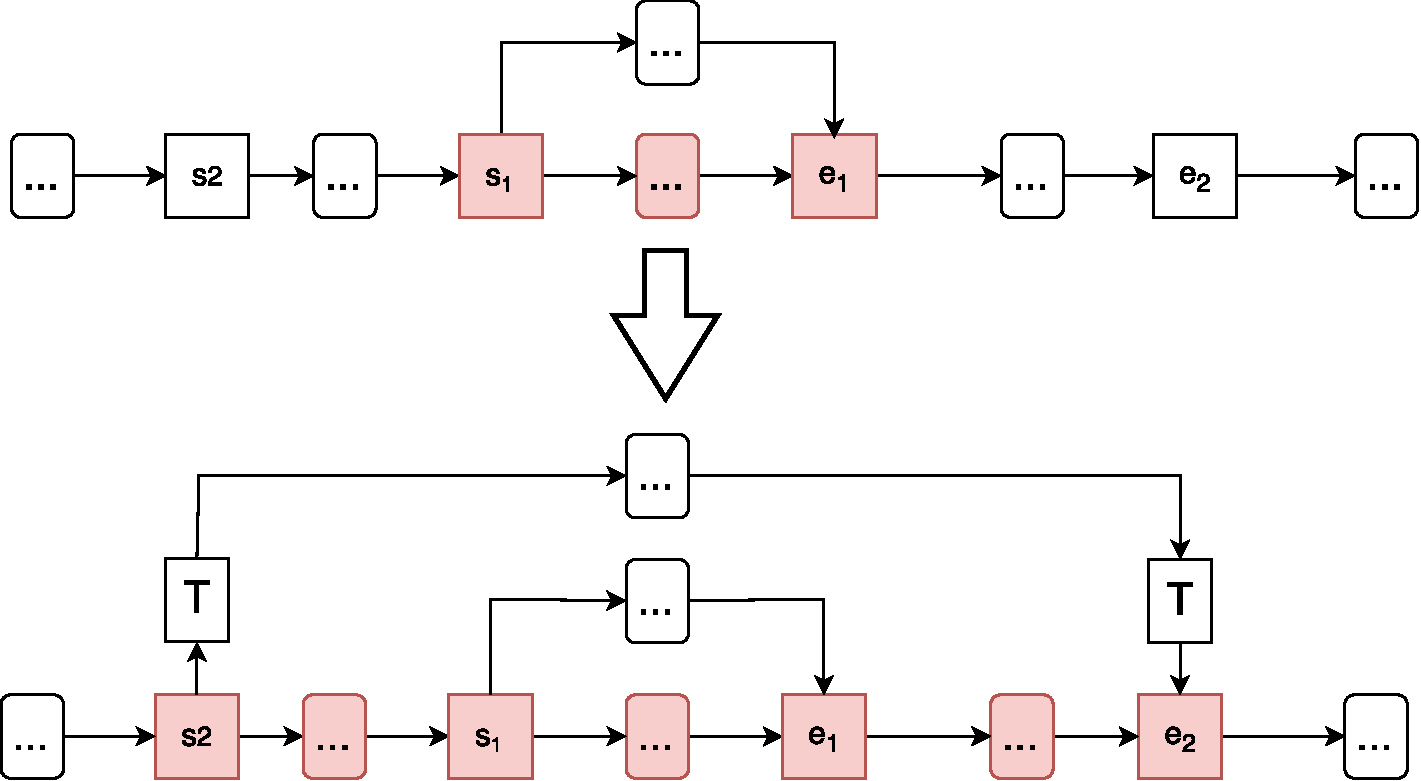
\includegraphics[width=\textwidth]{conflict1.pdf}
\caption{How Push Around handles the case, where we insert a new line that covers the entirety of an old line}
\label{fig:pusharound1}
\end{figure}

There is also the case, where the new line is covered by the old line entirely. In this case, we use the transformation in \cref{fig:pusharound2}. Here we do not need to append any transport module, as we move up through the already existing modules, which we would otherwise intersect with. 

In the cases where the new entirely intersects the old it will add transport modules where needed, or otherwise guide itself vertically through modules that already exists. These examples only show the case, where a single old line is placed above the main line, from which we branch off. In the case of more line levels, the new line will simply climb vertically until it finds a level where it may be placed without intersection. 

Push around is the intersect handling, we use when inserting new lines as a result of anti-serialization. This is chosen as there is no need to keep this new line close to \Gamma_0, from which it sprouted. 

\begin{figure}[H]
\centering
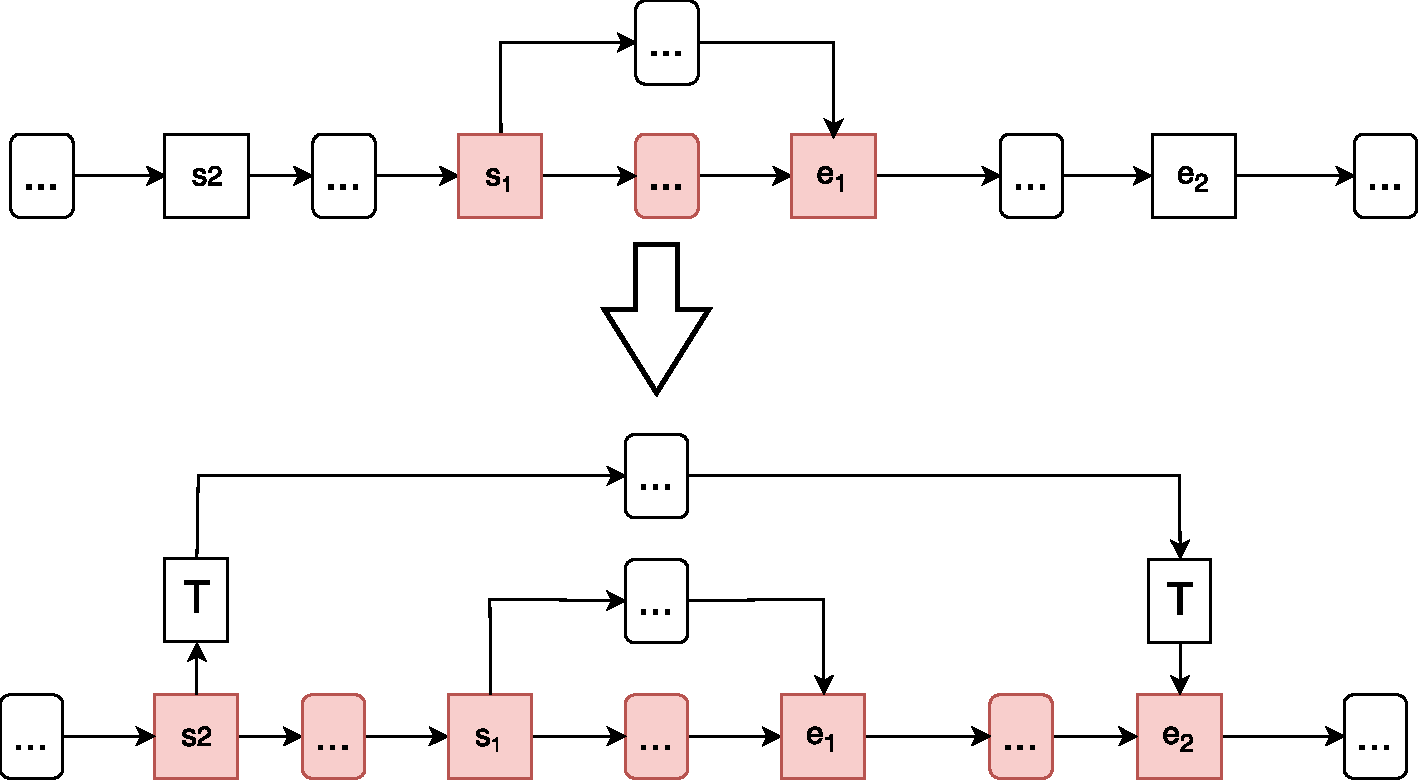
\includegraphics[width=\textwidth]{conflict2.pdf}
\caption{How Push Around handles the case, where we insert a new line that is covered by the entirety of an old line}
\label{fig:pusharound2}
\end{figure}

\subsection{Push Beneath} \label{ssec:pbeneath}
The other type of intersect handling that we use is called Push Beneath. Here we do the opposite of Push Around and handle intersection conflicts by placing the new line, where we want to place it and then moving vertically any old lines that may intersect. If this move creates another intersection we simply move the lines which we pushed into. This is done until no intersections remain. 

In the case where the new line is covered entirely by the old line we avoid intersection as in \cref{fig:pushunderneath1}. By pushing the new line up one level, we intersect the old, which needs to move up as well. This warrants that the old line gets support from transport modules.

\begin{figure}[H]
\centering
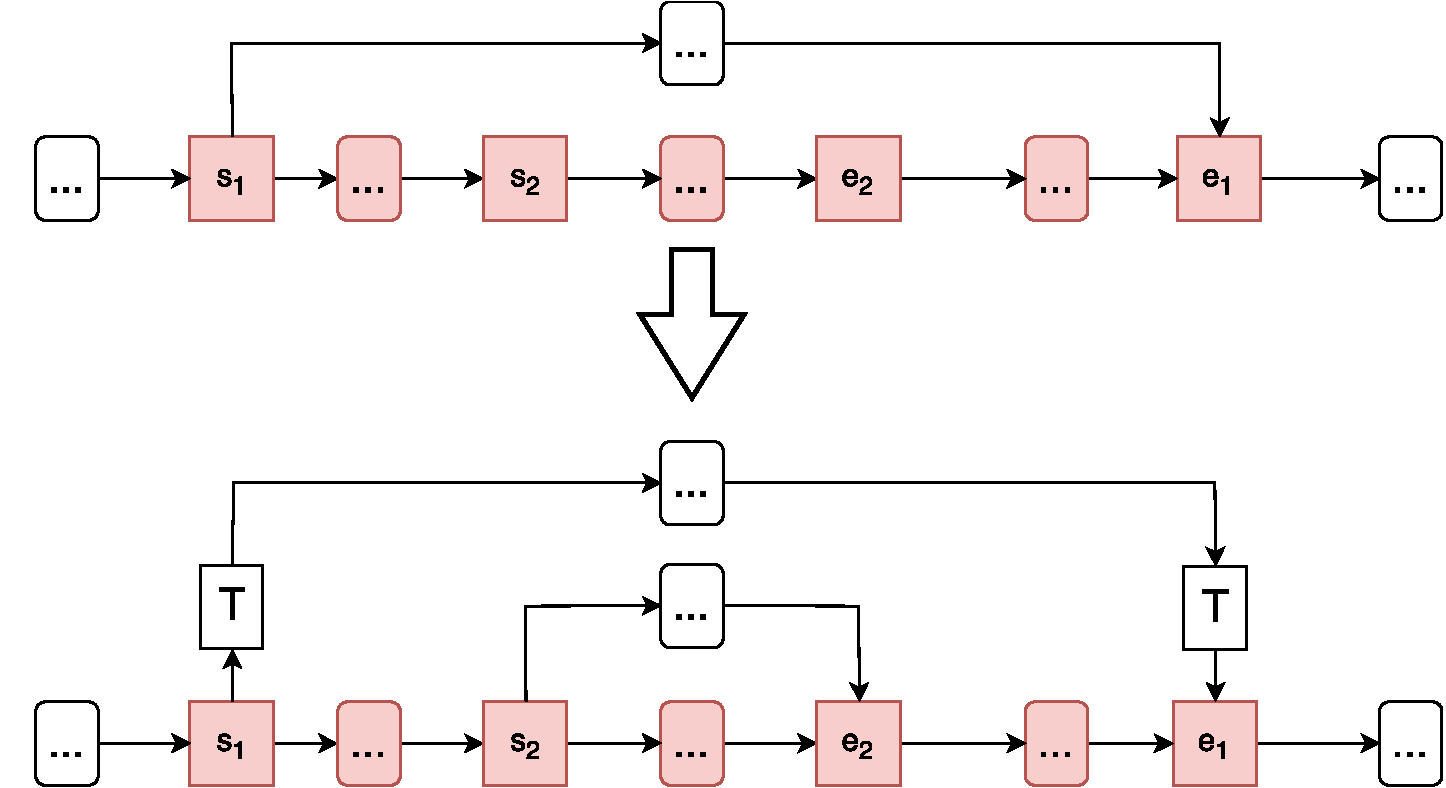
\includegraphics[width=\textwidth]{conflict3.pdf}
\caption{How Push Underneath handles the case, where we insert a new line that is covered entirely by an old line}
\label{fig:pushunderneath1}
\end{figure}

In the case, where the new line covers the old, we handle intersection as in \cref{fig:pushunderneath2}. As we push up the new line, we need to push up the old. However, we need not use transport modules to reconnect the old line, instead it can be reached by flowing vertically through the new line.

Again, the cases where there is a partial intersection between old and new line is easy to imagine. If the moving up of an old line creates a new intersection, we just move up the line that was already set in place. This is done until no more intersections occur. When this has been done, some old lines may have been disconnected from their main line. However, as these vertical connections are still included in either the $Start$ or $End$ function, transport modules may be appended, until a path has been recreated.  

As can be seen, Push Underneath functions in a manner opposite to Push Around. We decide to use it, when handling intersections that occur as a result of a parallel transformation. We want our parallel lines to be close to the line, which it sprouted from. Otherwise we may not reap the benefits of adding extra modules. This is not needed as much, when doing anti-serialization, which is why we use Push Around for that instead.

\begin{figure}[H]
\centering
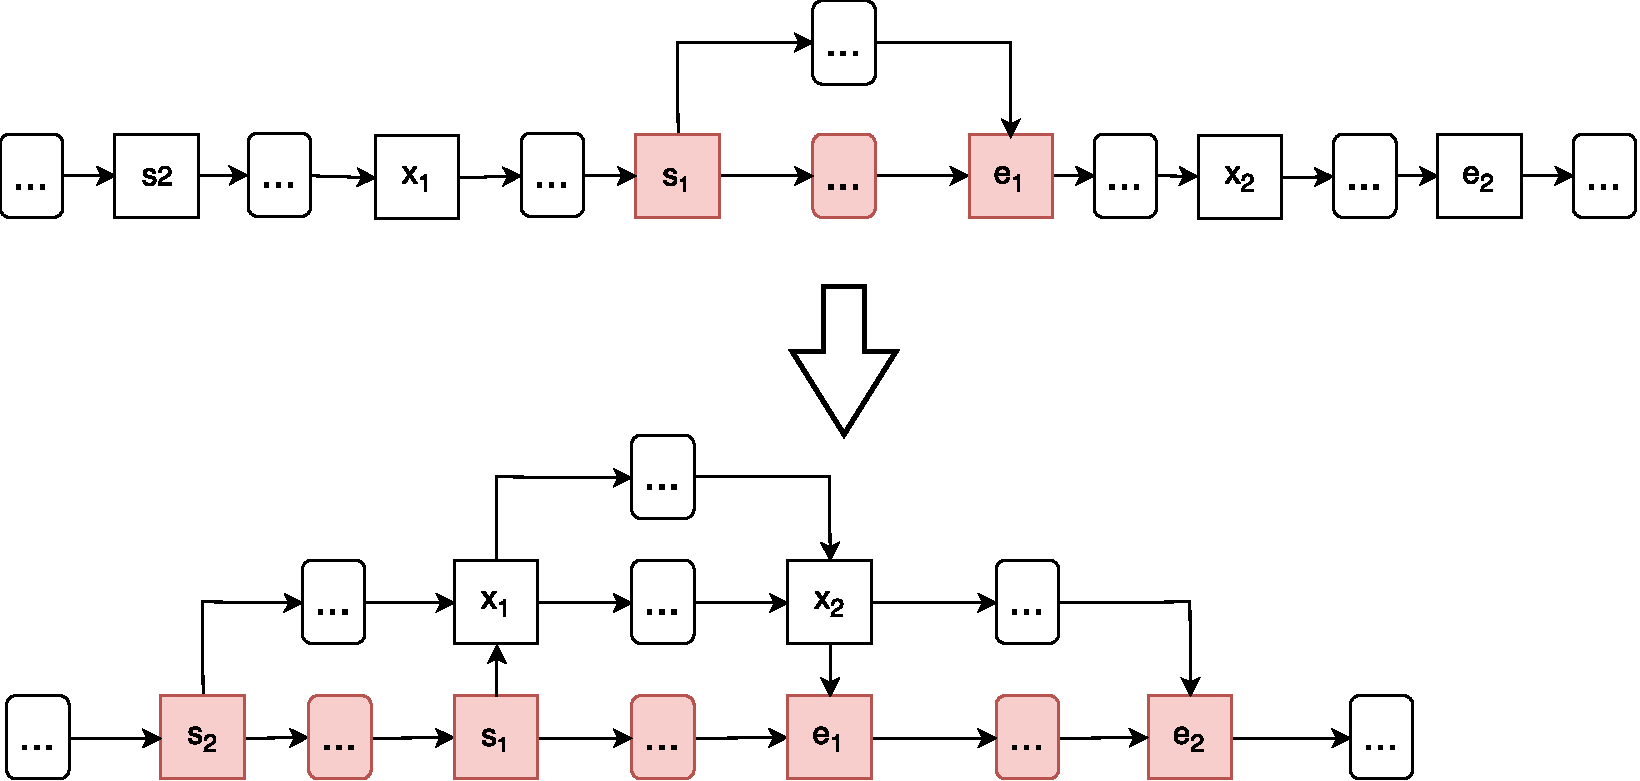
\includegraphics[width=\textwidth]{conflict4.pdf}
\caption{How Push Underneath handles the case, where we insert a new line that entirely covers an an old line}
\label{fig:pushunderneath2}
\end{figure}

 









